\documentclass[11pt, spanish]{article}
\usepackage[spanish]{babel}
\selectlanguage{spanish}
\usepackage[utf8]{inputenc}
\usepackage{graphicx}
\usepackage{mathtools}
\usepackage{tabularx}
\usepackage[font=small,labelfont=bf]{caption}
\usepackage{subcaption}
\usepackage{authblk}
\usepackage{natbib}
\usepackage{multirow}
\usepackage{color}   % For color text: \color command

\captionsetup[table]{name=Tabla}
\renewcommand{\thetable}{\Roman{table}}
\newcommand{\mean}[1]{\left\langle#1\right\rangle}
%\newcommand{\eqref}[1]{Ec.~\ref{#1}}

\graphicspath{
{figuras/},
} % Lugar donde encontrar las figuras generales (se puede poner uno en cada cap{\'{\i}}tulo)

\begin{document}
\begin{titlepage}
    \centering
    {\scshape\LARGE Universidad de Buenos Aires \par}
    \vspace{1cm}
    {\scshape\Large Informe 3:\par}

    \vspace{1.5cm}
    {\scshape\Large\par}
    {\huge\bfseries  Comunidades\par}
    \vspace{2cm}
    {\Large\itshape Ra\'ul Barriga\par}
    {\Large\itshape Mariela Celis\par}
    {\Large\itshape Jimmy Mas\'ias\par}
    {\Large\itshape Sebast\'ian Pinto\par}

    \vfill

    \vfill

                                                    % Bottom of the page
    {\large \today\par}
\end{titlepage}

    %--- tabla de contenidos
    \tableofcontents

    \section{Partición en clusters}

\begin{figure}
\centering
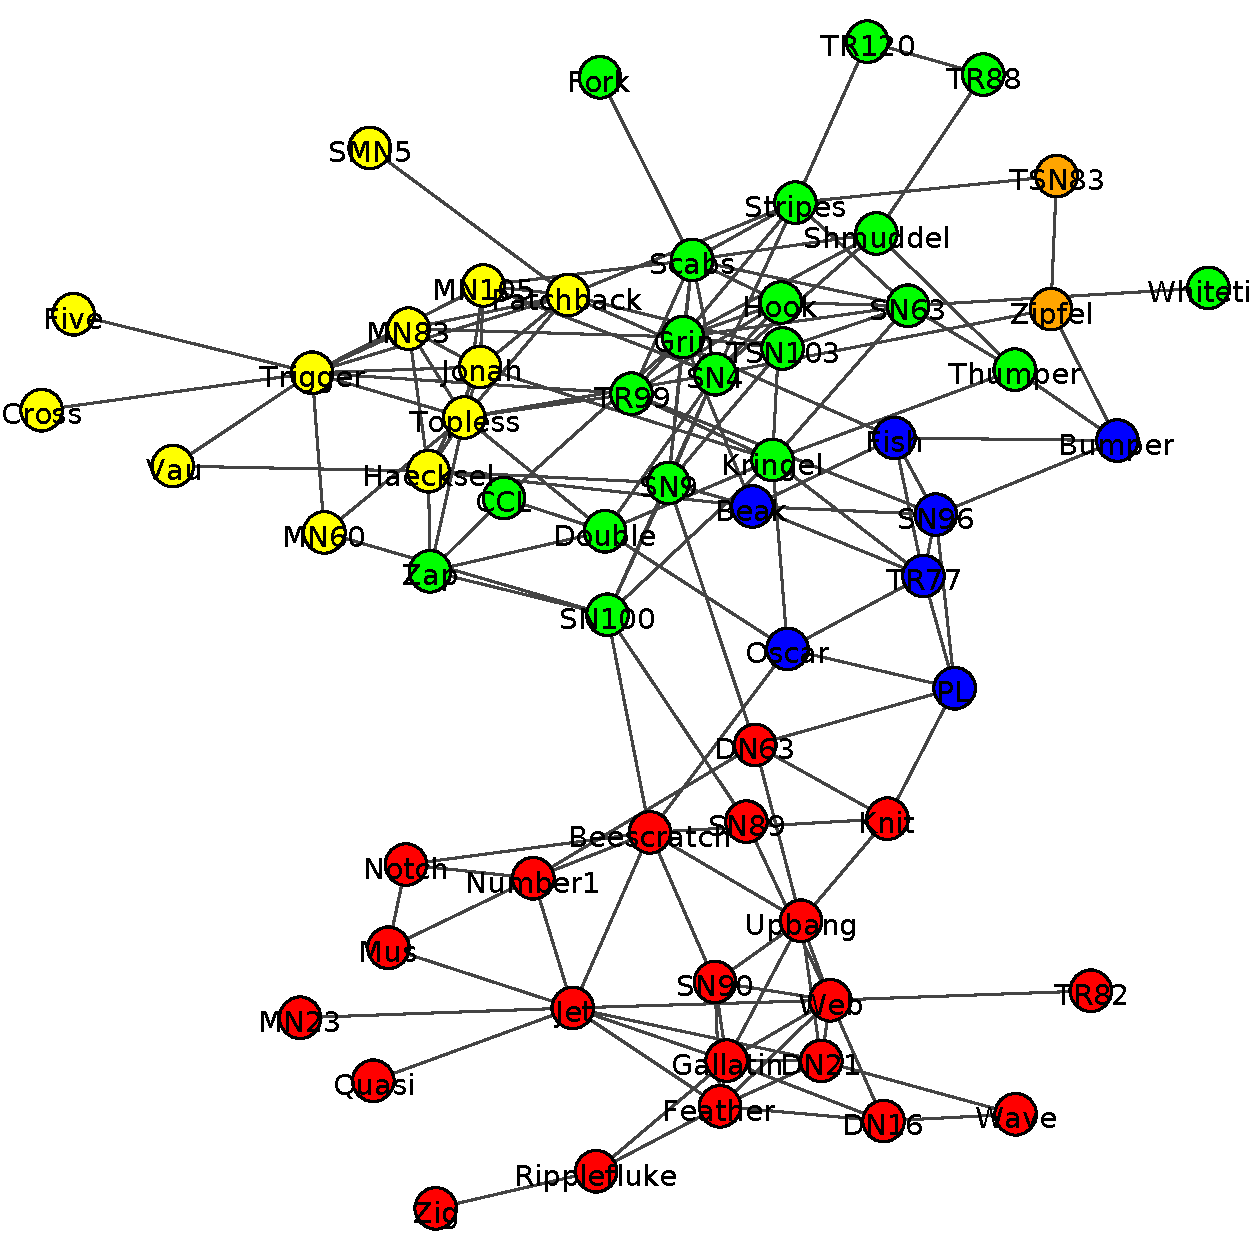
\includegraphics[scale = 0.2]{figuras/Edge_betweenness}
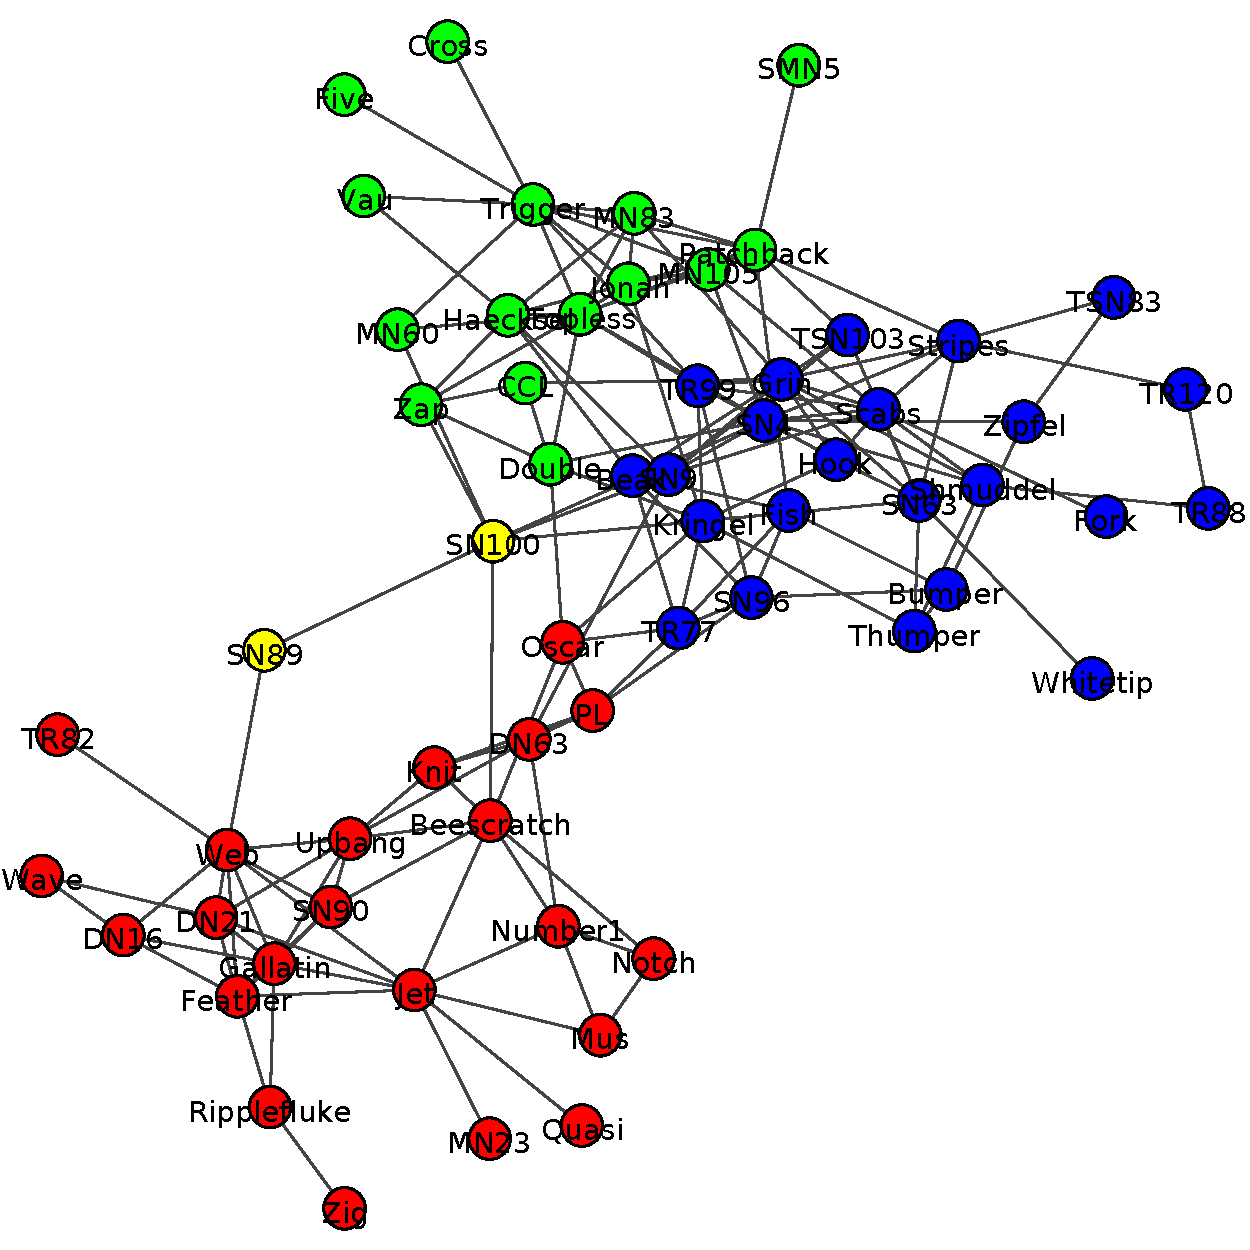
\includegraphics[scale = 0.2]{figuras/Fast_greedy} \\
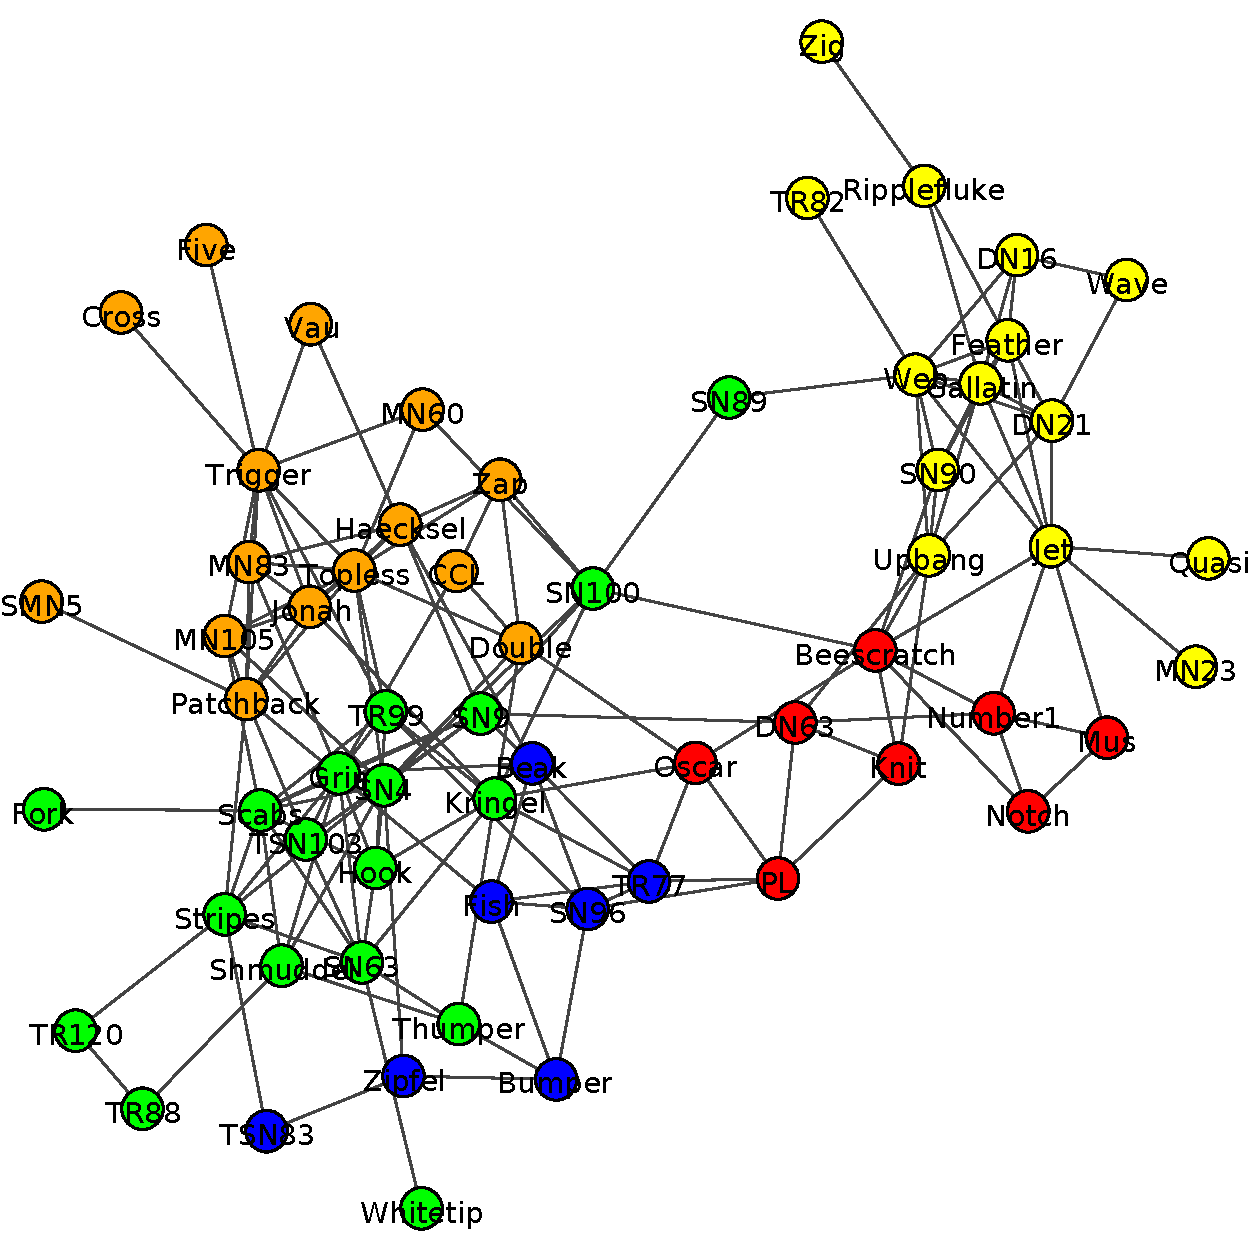
\includegraphics[scale = 0.2]{figuras/Louvain}
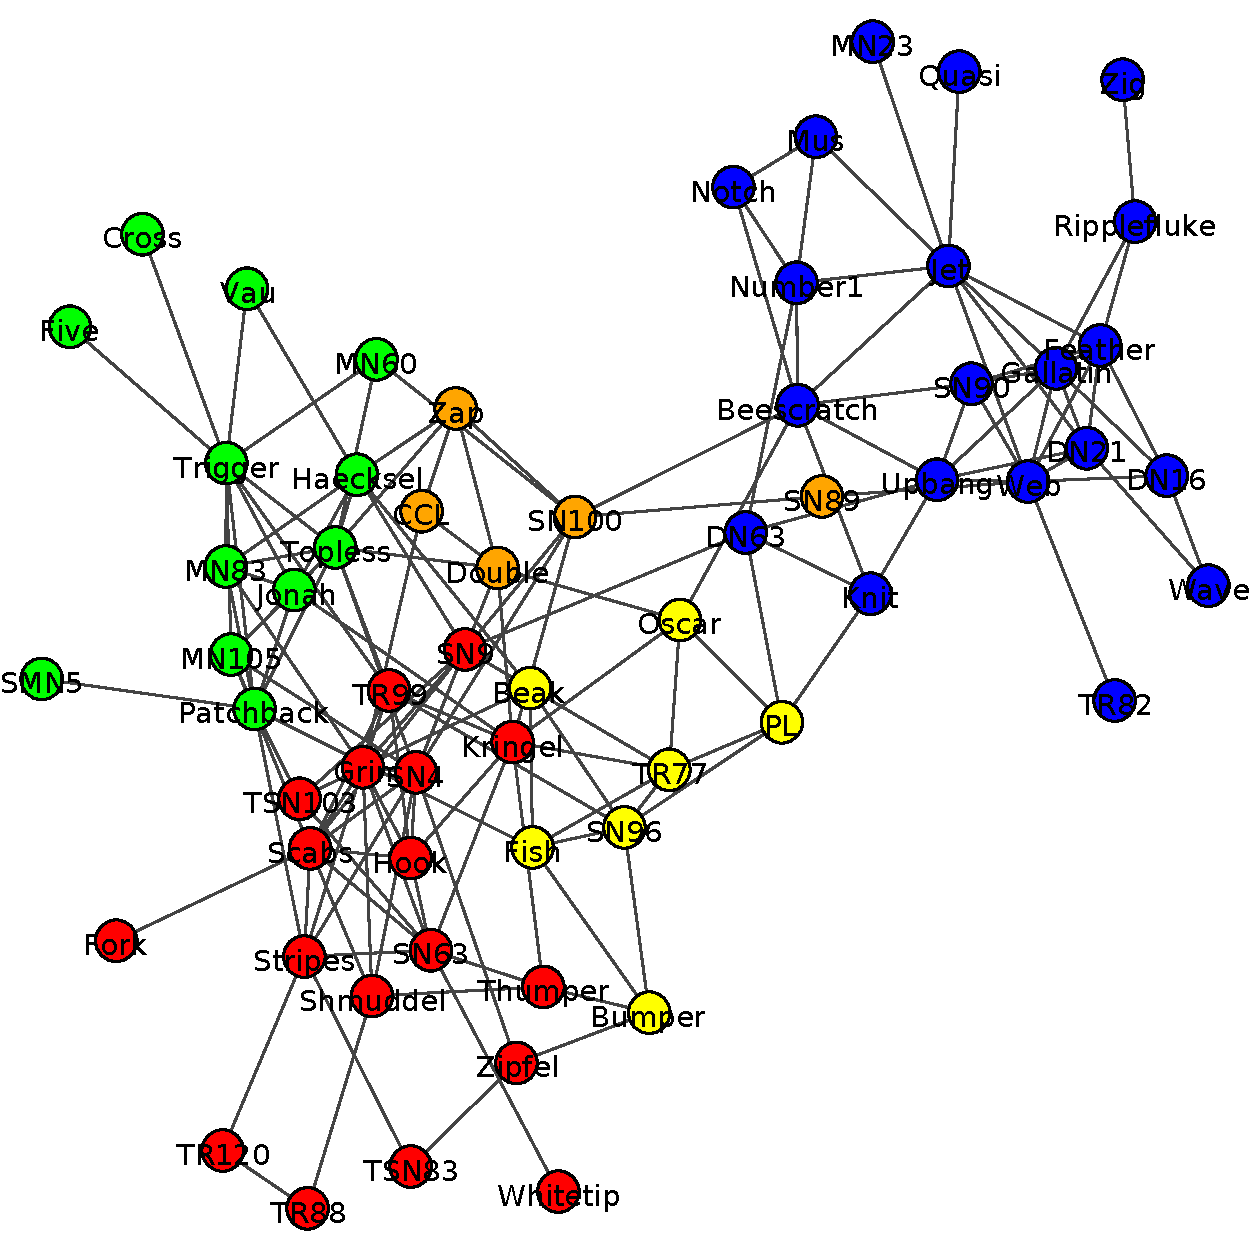
\includegraphics[scale = 0.2]{figuras/Infomap}
\caption{Layouts indicando el cluster asignado por cada algoritmo.}
\label{fig:Layouts_clusters}
\end{figure}

\section{Modularidad}

\begin{table}
\centering
\begin{tabular}{c c}
\hline \hline
Algoritmo & Modularidad \\
\hline
Fast greddy & 0.495 \\
Infomap & 0.529 \\
Edge-betweenness & 0.519 \\
Louvain & 0.519 \\
\hline\hline
\end{tabular}
\caption{Modularidad de las particiones dadas por diferentes algoritmos.}
\label{table:Modularidad}
\end{table}


\begin{figure}
\centering
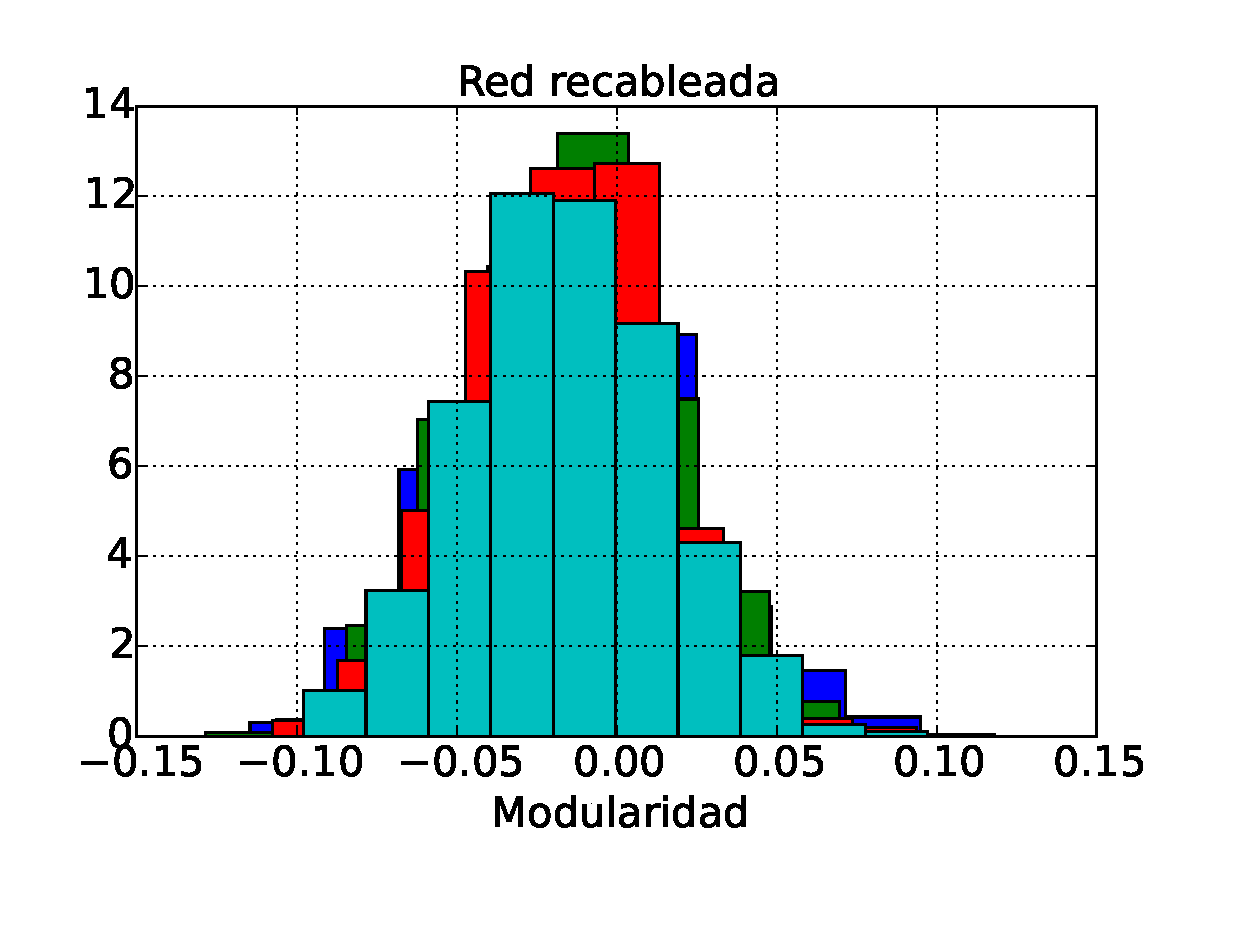
\includegraphics[scale = 0.5]{figuras/Modularidad_random}
\caption{Modularidad recableando en forma aleatoria, manteniendo la categoría dada por los algoritmos de detección de particiones.}
\label{fig:Modularidad_random}
\end{figure}

    \input{raul}
    \input{mariela}
    %--- commands/defs
\newcommand{\img}[2]{\includegraphics[scale=#1]{{#2}.png}}
\newcommand{\jmc}[1]{{\color{red}{(JM: #1)}}}   % jimmy comment



%--- doc
\section{Relaci\'on entre g\'enero y estructura de comunidades}
\label{sec:info_mutua}

Para cuantificar la relaci\'on entre el g\'enero de los delfines y la estructura de comunidades que fueron deducidas por los diferentes algoritmos (e.g. {\it Greedy}), empleamos la definici\'on de {\it Informacion Mutua}:

\begin{align}
    I(\{c1\},\{c2\}) = \sum_{c1,c2} p(c1,c2) log \frac{p(c1,c2)}{p(c1) p(c2)},
\label{eq:info_mutua}
\end{align}

donde $c1$ y $c2$ son etiquetas de las comunas del grafo.
Y definimos la informaci\'on mutua normalizada,

\begin{align}
    I_n (\{c1\},\{c2\}) &= 2 I(\{c1\},\{c2\}) / ( H(\{c1\}) + H(\{c2\}) ) \nonumber \\
    H(\{c1\}) &= - \sum_{c1} p(c1) log(p(c1))
\label{eq:info_mutua_norm}
\end{align}

Las comunas construidas en el presente grafo fueron deducidas usando los algoritmos {\it greedy, betweenness, infomap} y {\it louvain}.
La definici\'on \ref{eq:info_mutua} cuantifica cuanto se departa la informaci\'on real del grafo, respecto de la cantidad de informaci\'on que brinda una grafo cuyas comunas estan descorrelacionadas del g\'enero. \jmc{che Seba, a ver si esto tiene sentido}.
En el caso particular en que $\{c1\}$ y $\{c2\}$ son el mismo conjunto, obtenemos la informaci\'on mutua normalizada $I_n=1$.


\begin{figure}
    \centering
    \img{0.5}{p12_greedy}
    \img{0.5}{p12_betweenness}
    \img{0.5}{p12_infomap}
    \img{0.5}{p12_louvain}
    \caption{
    Valores de las matrices de probabilidad conjunto para los algoritmos {\it greedy} (izquierda, arriba) {\it betweenness} (derecha, arriba), {\it infomap} (izquierda, abajo) y {\it louvain} (derecha, abajo). 
    }
\label{fig:prob_conj}
\end{figure}


\begin{figure}
    \centering
    \img{0.6}{hist_sort_sex}
    \caption{
    Distribuci\'on del n\'umero de enlaces entre g\'eneros diferentes, para diferentes realizaciones de sorteo del sexo de los nodos de la red (manteniendo constante el n\'umero de masculinos y femeninos por separado).
    La l\'inea negra muestra el valor que corresponde a la red original que caracterizamos en este trabajo.
    La zona sombreada en celeste representa la regi\'on que cubre la desviaci\'on est\'andar respecto de la media.
    El valor de la red original (o real) se aparta $1 \sigma$ respecto del centro de la distribuci\'on, lo cual muestra una tendencia a la existencia de comunas que tienen muchos ejemplares de un sexo en particular.
    Esto es consistente con el bajo valor ($\ll 1$) de la informaci\'on mutua $I_n$ (ver ec. \ref{eq:info_mutua_norm} y Secc. \ref{sec:info_mutua}).
    }
\label{fig:hist_sort_sex}
\end{figure}

%EOF


%\bibliographystyle{plainnat}
%\bibliography{biblio}

\end{document}
